\chapter{\IfLanguageName{dutch}{Stand van zaken}{State of the art}}
\label{ch:stand-van-zaken}

% Tip: Begin elk hoofdstuk met een paragraaf inleiding die beschrijft hoe
% dit hoofdstuk past binnen het geheel van de bachelorproef. Geef in het
% bijzonder aan wat de link is met het vorige en volgende hoofdstuk.

% Pas na deze inleidende paragraaf komt de eerste sectiehoofding.

% Dit hoofdstuk bevat je literatuurstudie. De inhoud gaat verder op de inleiding, maar zal het onderwerp van de bachelorproef *diepgaand* uitspitten. De bedoeling is dat de lezer na lezing van dit hoofdstuk helemaal op de hoogte is van de huidige stand van zaken (state-of-the-art) in het onderzoeksdomein. Iemand die niet vertrouwd is met het onderwerp, weet nu voldoende om de rest van het verhaal te kunnen volgen, zonder dat die er nog andere informatie moet over opzoeken \autocite{Pollefliet2011}.

% Je verwijst bij elke bewering die je doet, vakterm die je introduceert, enz. naar je bronnen. In \LaTeX{} kan dat met het commando \texttt{$\backslash${textcite\{\}}} of \texttt{$\backslash${autocite\{\}}}. Als argument van het commando geef je de ``sleutel'' van een ``record'' in een bibliografische databank in het Bib\LaTeX{}-formaat (een tekstbestand). Als je expliciet naar de auteur verwijst in de zin, gebruik je \texttt{$\backslash${}textcite\{\}}.
% Soms wil je de auteur niet expliciet vernoemen, dan gebruik je \texttt{$\backslash${}autocite\{\}}. In de volgende paragraaf een voorbeeld van elk.

% \textcite{Knuth1998} schreef een van de standaardwerken over sorteer- en zoekalgoritmen. Experten zijn het erover eens dat cloud computing een interessante opportuniteit vormen, zowel voor gebruikers als voor dienstverleners op vlak van informatietechnologie~\autocite{Creeger2009}.
\section{Progressive web applicatie}
In deze sectie wordt er beschreven wat een progressive web applicatie allemaal extra nodig heeft naast een ontwikkelde website(\cite{PWA_EXTRA_FEATURES})(\cite{PWA_EXTRA_FEATURES_2}).

\subsection{Service worker}
Het eerste item dat een progressive web applicatie nodig heeft is een service worker. Deze zorgt ervoor dat de website alle aanvragen voor externe data kan opslaan, beter bekend als data caching. De aanvragen worden doorgestuurd naar de service worker die deze dan op zijn beurt haalt van de externe databron online of de lokale gecachte data. De service worker maakt deze beslissing op basis van de ingestelde strategie. Er zijn momenteel vijf strategieën die gebruikt kunnen worden met workbox (\cite{WORKBOX_STRATEGIES}). Deze strategieën zijn stale white revalidate, offline first, online first, network only en cache only.

\subsubsection{Stale-While-Revalidate}
Deze strategie zorgt ervoor dat de gebruiker zo snel mogelijk een antwoord heeft op de aangevraagde data. Dit gebeurd doordat de service worker eerst de gecachte data zal weergeven als deze beschikbaar is. Indien er geen gecachte data is zal de service worker de aanvraag via het netwerk doen. Met het antwoord van het netwerk zal de cache dan weer geüpdatet worden met de laatste versie van de data.

\begin{figure}[!h]
	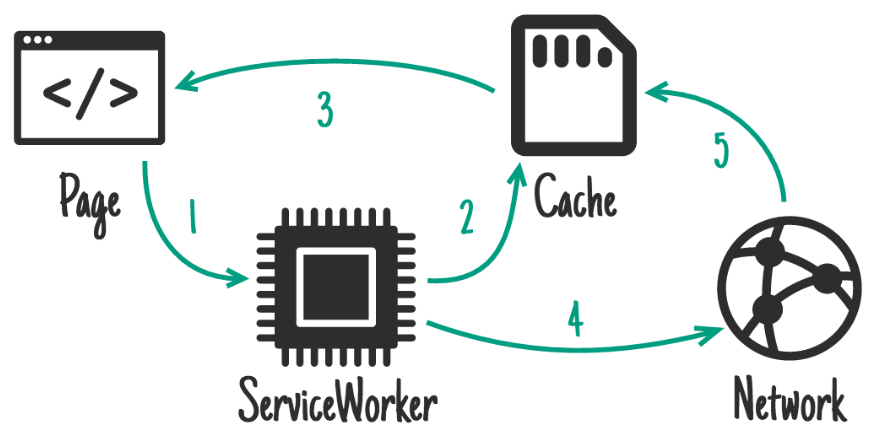
\includegraphics[width=200px]{ServiceWorker/StaleWhileRevalidate}\centering
	\caption{Voorstelling stale-while-revalidate strategie}
\end{figure}

\subsubsection{Offline first}
Bij deze strategie gaat de service worker kijken of de aangevraagde data al reeds gecached is op het apparaat. Als de data al reeds opgeslagen is op het apparaat, dan gebruikt de service worker de data die al reeds gecached is. Is er reeds geen data opgeslagen dan gaat de service worker via het netwerk de externe data opvragen. Eén van de grote nadelen van deze strategie is dat de externe data niet altijd up to date is.

\begin{figure}[!h]
	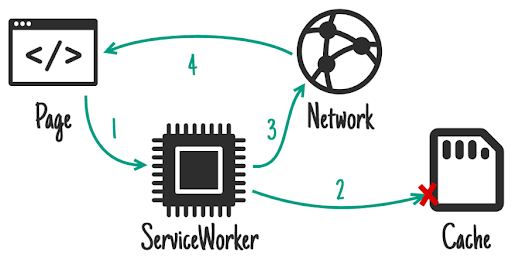
\includegraphics[width=200px]{ServiceWorker/OfflineFirst}\centering
	\caption{Voorstelling offline first strategie}
\end{figure}

\subsubsection{Online first}
Bij online first zal de service worker eerst de aanvraag doen via het netwerk. Als er geen netwerkverbinding is zal de service worker de gecachte data weergeven indien deze aanwezig is. Om deze reden moet er altijd een netwerkverbinding zijn om alle data binnen te halen voordat de applicatie offline de data kan weergeven. Met deze strategie is de externe data altijd up to date indien er een netwerkverbinding is.

\begin{figure}[!h]
	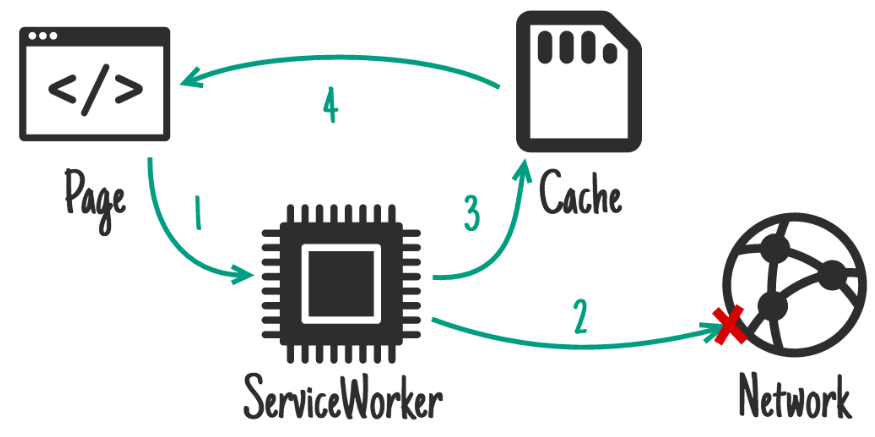
\includegraphics[width=200px]{ServiceWorker/OnlineFirst}\centering
	\caption{Voorstelling online first strategie}
\end{figure}

\subsubsection{Network Only}
Network only is een strategie die de externe data enkel maar via het netwerk zal ophalen. Als deze niet beschikbaar is zal de gecachte data ook niet weergegeven worden.

\begin{figure}[!h]
	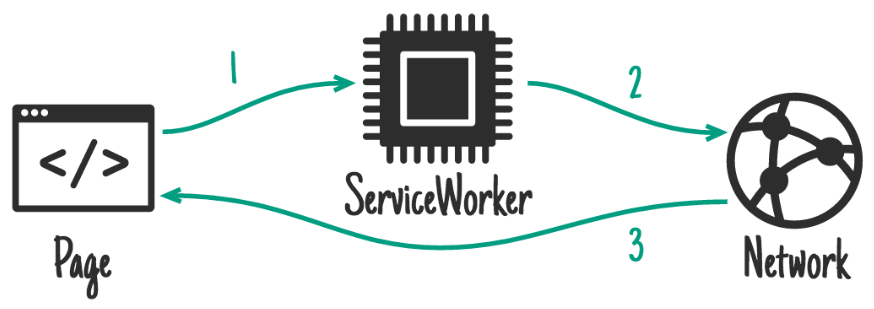
\includegraphics[width=200px]{ServiceWorker/NetworkOnly}\centering
	\caption{Voorstelling network only strategie}
\end{figure}

\subsubsection{Cache Only}
Cache only werkt alleen maar met de gecachte data. Deze haalt geen externe data gaan via het netwerk. Deze strategie kan gebruikt worden voor sites die geen externe data nodig hebben zoals een rekenmachine.

\begin{figure}[!h]
	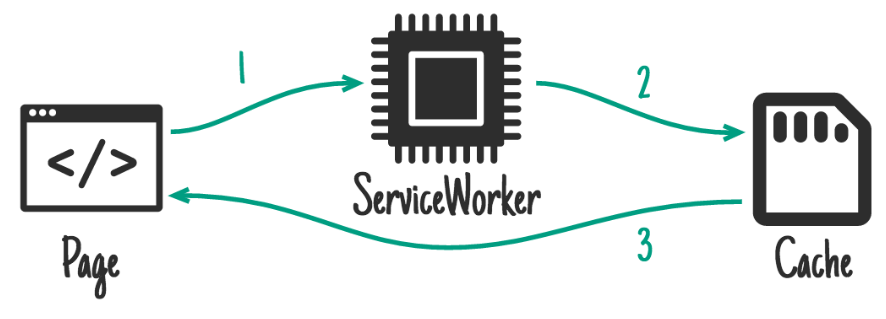
\includegraphics[width=200px]{ServiceWorker/CacheOnly}\centering
	\caption{Voorstelling cache only strategie}
\end{figure}

\subsection{Manifest}
Het tweede item dat een progressive web applicatie nodig heeft is een manifest \cite{MANIFEST}. Dit is een bestand met alle informatie die nodig is om de applicatie draaiende te houden eens deze geïnstalleerd is op het apparaat. Deze informatie bevat maar is niet gelimiteerd tot de auteur, het icoon en de versie.

\subsubsection{Auteur}
De naam van de auteur van de applicatie. Deze kan ook de naam van het bedrijf zijn.

\subsubsection{Icoon}
Het icoon waarmee de applicatie wordt weergegeven bij de applicaties op het apparaat. Er kunnen verschillende iconen meegegeven worden. Deze kunnen dienen voor de verschillende besturingssystemen, zodat er bijvoorbeeld een uniek icoon is voor apple en android. De iconen kunnen ook een verschillende grootte hebben, dit zorgt ervoor dat het icoon goed zichtbaar is op elk scherm van de verscheidene apparaten.

\subsubsection{Versie}
De versie van applicatie kan ook ingesteld worden door de manifest file. Zo weet de gebruiker welke versie van de applicatie er geïnstalleerd is op zijn apparaat.

\section{Frameworks}
\subsection{Wat is een framework ?}
Een Framework is een geheel van softwarecomponenten dat gebruikt kan worden bij het programmeren van applicaties. Ook de afspraken over hoe die componenten gebruikt worden binnen een groep ontwikkelaars en welke code-standaarden en bibliotheken gebruikt worden kunnen onderdeel zijn van een framework. Het framework bepaalt welke software er binnen een organisatie wordt gebruikt en op welke manier (\cite{WIKI_FRAMEWORK}).

\subsection{Requirements}
Wegens we de performance willen vergelijken tussen de twee frameworks zullen we gebruik maken van dezelfde backend applicatie namelijk google firebase.

De requirements voor de web applicatie zijn de volgende:

\begin{itemize}
	\item Service worker
	\item Manifest
	\item Router
	\item Store
	\item Data binding
\end{itemize}

De requirements voor de native applicatie zijn de volgende: 
\begin{itemize}
	\item Cross-platform
	\item Data binding
\end{itemize}

\subsection{Gekozen frameworks}
\subsubsection{Progressive web applicatie}
Er zijn verschillende frameworks voor een progressive web applicatie te ontwikkelen, maar op basis van bovenstaande requirement is er gekozen voor Vue.js in combinatie met Nuxt.js voor het creëren van de progressive web applicatie.
Andere mogelijkheden zijn (\cite{FRAMEWORKS_PROGRESSIVEWEBAPPS}) Angular, React, Ionic en Polymer.


\paragraph{Angular 2+}
Deze heeft ook een package om de site naar een progressive web applicatie te transformeren.
De reden waardoor angular niet geselecteerd werd, is omdat er een basiskennis van typescript aanwezig moet zijn voordat er een applicatie kan gebouwd worden. Anderzijds werd er beslist om met Vue te werken wegens dit het best beoordeelde framework is (\cite{VUE_POPULARITY}).

\paragraph{React}
React is geen officieel framework maar een library. Toch wordt deze opgenomen in de mogelijkheden omwille dat er een progressive web applicatie ontworpen kan worden met react. Deze werd niet geselecteerd omdat de programmeur een kennis van JSX hebben om react te kunnen gebruiken.

\paragraph{Ionic}
Ionic werd niet geselecteerd omwille dat de applicatie frequent moet geüpdatet worden om mee te kunnen met de laatste veranderingen van het framework (\cite{ICONIC}). Hierdoor kan de applicatie vrij snel verouderd worden. Als de site gebruik maakt van een verouderde package kan deze de site laten vastlopen.

\paragraph{Polymer}
De reden waarom polymer niet geselecteerd werd is dat het niet search engine optimised is (\cite{POLYMER}). Vervolgens heeft deze ook een hoge herlaadtijd voor de site.

\subsubsection{Native applicatie}
Om de native applicatie te ontwikkelen hebben is er gekozen voor het framework kotlin. Andere frameworks die in aanmerking kwamen waren Java en Xamarin.

\paragraph{Java}
Java is een populair framework onder de developers. Deze wordt nog altijd gebruikt voor allerhande applicaties, van bureaublad applicaties tot android applicaties. Kotlin heeft vele aspecten van java maar heeft deze beter gemaakt. Om die reden wordt de performantie hoger bij het gebruik van het Kotlin framework dan het Java framework. (\cite{KOTLIN_VS_JAVA})

\paragraph{Xamarin}
Xamarin werd niet geselecteerd door dat de performantie op het android platform niet optimaal is. De performantie op ios is veel beter. Bijkomend zijn er maar een paar ondersteunende Integrated development environments (IDE’s). Xamarin heeft ook geen ondersteuning voor android xml files die nodig zijn voor de opmaak. Om deze reden worden veel fouten gemaakt bij de xml bestanden tijdens de programmatie van de applicatie. (\cite{KOTIN_VS_XAMARIN}).


\subsection{Browserondersteuning}
Een browser moet een PWA kunnen ondersteunen voor deze uitgevoerd kan worden. Omwille dat de PWA functionaliteit nog maar vier jaar oud is is deze nog niet overal geïmplementeerd. Hieronder wordt bekeken of de bekendste browsers de PWA functionaliteit al ondersteunen. De ondersteuning van de PWA functionaliteit in Safari kon niet gevalideerd worden wegens dat er geen apparaat beschikbaar was met Safari.

\subsubsection{Chrome}
Wegens dat de PWA functionaliteit ontwikkeld is door Google is chrome de eerste browser die deze ondersteund. Chrome kan de PWA zowel op mobiel als op computer gebruiken. Eens deze applicatie geïnstalleerd is op mobiel zal deze verschijnen tussen de andere applicaties, op de computer zal deze verschijnen bij het tabblad chrome://apps.

\subsubsection{Firefox}
Firefox ondersteunt standaard de PWA functionaliteit niet op de computer. Deze kan wel aangezet worden door een paar instellingen te wijzigen.
Op mobiel ondersteunt Firefox de PWA functionaliteit wel met de Firefox Browser app, dit betekent dat de applicatie installeerbaar is. Na installatie is er een icoon te zien op het home scherm, maar niet in de applicaties zoals bij google chrome.

\subsubsection{Opera}
De PWA functionaliteit wordt helaas nog niet ondersteund op de computer. De service worker daarentegen wel. Deze zorgt ervoor dat de site nog beschikbaar is als het internet uitvalt. 
De mobiele versie van Opera (Opera Browser with free VPN) ondersteunt de PWA functionaliteit wel. Na installatie zal er net zoals bij de firefox browser een icoon te zien zijn op het home scherm maar zal deze niet voorkomen in de applicaties op het apparaat.
Verder werd er ook gekeken naar de nieuwe mobiele applicatie Opera Touch. Deze ondersteunt PWA functionaliteit niet.

\subsubsection{Safari}
Safari ondersteunt sinds IOS 11.3 de PWA functionaliteit. Na de installatie is de applicatie terug te vinden bij de andere applicaties op het home scherm. Aangezien de applicatie te installeren is via de browser heeft de applicatie geen quality test van apple ondergaan. Apple heeft een paar limitaties opgelegd aan deze soort applicaties zodat het apparaat nog altijd optimaal zou beschermd zijn. Een paar van deze limitaties zijn dat de applicatie maximaal 50 megabyte aan data mag verzamelen offline, er geen communicatie kan ontstaan tussen verschillende Apple-services zoals app betalingen en er geen push notifications ondersteund worden (\cite{BROWSERSUPPORT_IOS}).

\subsection{Store}
Deze sectie geeft een breder inzicht of de PWA site toegevoegd kan worden in de app store en play store.

\subsubsection{Play Store}
Google heeft reeds in 2019 beslist om de PWA functionaliteit toe te voegen aan de store (\cite{PLAYSTORE}). Voor een PWA in de play store te kunnen toevoegen moet er een native applicatie met de nodige certificaten worden aangemaakt met in de applicatie een verwijzing naar de PWA site. Op deze manier zal de applicatie de laatste data tonen van de PWA site zonder elke versie te moeten opladen naar de play store. Enkel voor grote veranderingen binnen de applicatie zoals het icoon, het manifest bestand, en de TWA(Trusted Web Activity) moet er een nieuwe versie geupload worden naar de play store.

\subsubsection{App Store}
Voor je een PWA kan uploaden in de app store heb je een native wrapper nodig zoals Cordova. Deze zet de code om naar een Xcode project, dit draagt het nadeel met zich mee dat een PWA enkel op een MacOs apparaat kan geüpload worden in de store. (\cite{APPSTORE})
